\documentclass[12pt,a4paper]{report}

\usepackage[utf8]{inputenc}
\usepackage[spanish]{babel}
\usepackage{geometry}
\geometry{top=2.5cm, bottom=2.5cm, left=3cm, right=3cm}
\usepackage[colorlinks=true, linkcolor=blue, urlcolor=blue]{hyperref}
\usepackage{minitoc}
\usepackage{xcolor}
\usepackage{listings}
\usepackage{graphicx}

\definecolor{codegreen}{rgb}{0,0.6,0}
\definecolor{codegray}{rgb}{0.5,0.5,0.5}
\definecolor{codepurple}{rgb}{0.58,0,0.82}
\definecolor{backcolour}{rgb}{0.95,0.95,0.92}


\lstdefinestyle{estiloJava}{
	backgroundcolor=\color{backcolour},   
	commentstyle=\color{codegreen},
	keywordstyle=\color{blue}\bfseries,
	numberstyle=\tiny\color{codegray},
	stringstyle=\color{codepurple},
	basicstyle=\ttfamily\footnotesize,
	breakatwhitespace=false,         
	breaklines=true,                 
	captionpos=b,                    
	keepspaces=true,                 
	numbers=left,                    
	numbersep=5pt,                  
	showspaces=false,                
	showstringspaces=false,
	showtabs=false,                  
	tabsize=4,
	language=Java
}
\lstset{style=estiloJava}

\begin{document}
	
	\title{\Huge \textbf{Manual: De lo basico de Java hasta Spring}}
	\author{Christoper Zashiel Ramirez Alba}
	\date{\today}
	\maketitle
	

	\dominitoc 
	\tableofcontents 
	\newpage
	
	

\chapter{Tecnología de Java}


\minitoc 
\newpage 

\section{¿Que es Java?}

Java es un lenguaje de programación (Programming Lenguage), un entorno de desarrollo (Development Enviorenment) y de despliegue o en ingles se conoce como (Deployment Enviorenment).
Para los que vienen de C o C++, Java comparte una sintaxis similar con estos últimos lenguajes mencionados y como un entorno de desarrollo, Java provee herramientas como un compilador, interprete, un generador de documentos, paquetes de archivos de clases, etc.
Java usualmente se utiliza mucho para ser una representación de la realidad debido a que se usa un paradigma de programación llamada, \textbf{Programcion Orientada a objetos (Object-Oriented Programming)}.\\
En la modernidad Java se usa comúnmente como BackEnd para el World Wide Web(web) o en APIs (Aplication Programming Interface), también es usado en el Cloud, empresas y para las bases de datos (Big Data).
\subsection{Ventajas de Java}
\begin{itemize}
	\item Elimina el hecho de preocuparse sobre los apuntadores, algo que en C debes de tener mucho cuidado.
	\item Al ser su paradigma de Programación Orientada a Objetos, ayuda visualizar el programa mejor a la vida real. 
	\item Te permite optimizar mejor el código.
	\item Ayuda a la velocidad de desarrollo 
	\item Permite que el código se ejecute en múltiples sistemas operativos.
\end{itemize}
\subsection{Resumen de la historia de Java}

Java es un lenguaje de programación creado a principios de los años 90 por un equipo de ingenieros de Sun Microsystems liderado por James Gosling. Originalmente, el proyecto no estaba pensado para computadoras personales, sino para dispositivos electrónicos como televisores inteligentes. En sus inicios se llamó Oak, pero luego fue renombrado como Java.

El lenguaje fue presentado oficialmente en 1995 y rápidamente ganó popularidad gracias a su principal característica: “escribir una vez, ejecutar en cualquier lugar” (Write Once, Run Anywhere). Esto fue posible gracias a la Java Virtual Machine (JVM), que permite ejecutar programas en diferentes sistemas operativos sin necesidad de modificarlos.

Durante finales de los años 90 y principios de los 2000, Java se convirtió en uno de los lenguajes más utilizados para el desarrollo de aplicaciones empresariales, aplicaciones web y software en general. Su plataforma se expandió con tecnologías como Java SE, Java EE y Java ME.

En 2010, Oracle Corporation adquirió Sun Microsystems y pasó a ser responsable del desarrollo y mantenimiento de Java. Desde entonces, el lenguaje ha seguido evolucionando con nuevas versiones que mejoran su rendimiento, seguridad y facilidad de uso.

Hoy en día, Java sigue siendo uno de los lenguajes más importantes del mundo, ampliamente utilizado en aplicaciones empresariales, desarrollo backend, sistemas financieros y aplicaciones Android.

\section{Maquina Virtual de Java (Java Virtual Machine) JVM}
Es un software que emula una maquina real, es una maquina virtual que finge ser una maquina real dentro de la verdadera maquina real, suena redundante pero así funciona la JVM o en parte, el único propósito de este ultimo es simplemente ejecutar programas en Java. Gracia a JVM podemos compilar nuestros codigos de Java en muchos sistemas operativos porque esta maquina virtual es independiente a sistema, debido a que este genera Bytecode, que es el lenguaje que entiende el JVM.

\subsection{Garbage Collection}
El Garbage Collection se traduciría directamente como recolector de basura, empezare desde el principio: Cuando un programador escribe su codigo mediante un lenguaje este ultimo no es entendible por la maquina, se requiere de un proceso de compilado para que el lenguaje de programación se transforme a uno que entiende la maquina, osea en binario. Cada vez que haces un programa se asigna un bloque de memoria de tu código para luego ser ejecutado. Los lenguajes se manejan en niveles, de alto a bajo. \textbf{Mientras mas alto sea el nivel mas tardado es el tiempo de ejecución de tu programa}, Java es un lenguaje de alto nivel, es decir, es su sintaxis muy cercana al lenguaje humano, algo que en C no es así. \\

Los lenguajes como C o C++ te permiten usar memoria dinámica, usarla es de mucho cuidado porque puedes dejar bloques de memoria utilizados que para borrarlos resulta difícil o hasta imposible porque en las computadoras modernas existe una cantidad gigante de bloques de memoria. Java te permite quitarte ese peso pues gracias al Garbage Collection este desocupa los bloques de memoria que ya no utilice tu programa.

\subsection{Runtime Environment}

Esta sección dejare un diagrama de como corre un programa en java. 

\begin{figure}[htbp]
	\centering
	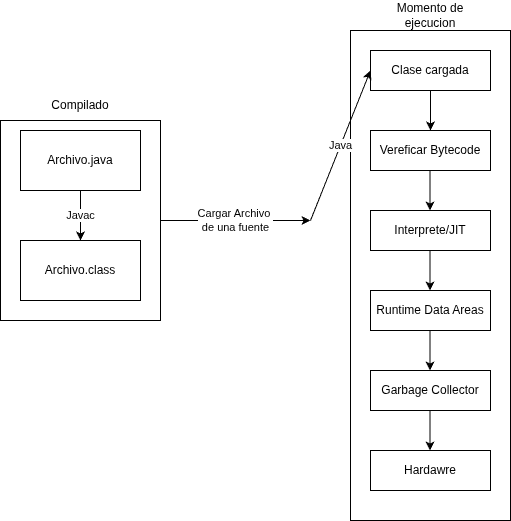
\includegraphics[width=0.8\textwidth]{Imagenes/Diagrama de JVM.png}
	\caption{Diagrama de JVM.}
	\label{fig:diagrama_base}
\end{figure}

Los archivos java son compilados y estos se transforman en Bytecodes pasa hacer archivos de tipo Class, luego el Bytecode es cargado en la memoria y se verifica que el código este en orden, es decir, evita errores de acceso ilegal de memoria o código corrupto, después se interpreta ejecutando linea por linea el Bytecode, pero al mismo tiempo JIT (Just-in-time Compiler), convierte el Bytecode en código maquina para mayor velocidad y el Garbage Collection se ejecuta en tiempo real para gestionar la memoria y así corre en tu Hardaware.\\

\section{Primeros pasos de Java}

En la fecha de hoy 3 de abril del 2026, uso como IDE a \textbf{VS Code} (Visual Studio Code), elegí este esta herramienta porque es ligera, muy flexible a extensiones y lo que me interesa y mas me gusta es que multilenguaje, la única desventaja es instalar las extensiones, pero mas adelante les daré para mi las mejore extensiones para programar en Java.\\
Tambien quiero mencionar otras IDE que son igual de buenas y merecen ser mencionadas: \textbf{IntelliJ IDEA} muy usada en la industria y desarrolladores de Java, \textbf{Eclipse} tiene la ventaja de ser muy personalizable para hacer código y \textbf{Apache NetBeans} muy amigable y facil de utilizar, no necesita instalar plugins.\\

Java tiene la ventaja de poderse instalar en multiples sistemas operativos, en mi caso uso Linux y como distribuidor Ubuntu en su versión 25.04, sin embargo también para los que vienen de Windows. Recomiendo que instalen VS Code y JDK (Java Development Kit) en la computadora que trabajes.

\subsection{Extensiones de Java}
A continuación daré las extensiones que mas he usado y que mas adelante usare para futuros proyectos.
\begin{enumerate}
	\item \textbf{Extension Pack for Java}: Proporciona un kit de herramientas muy útil para programar y son las siguientes.
	\begin{itemize}
		\item \textbf{Lenguage Support for Java}: Analiza tu código en tiempo real para ofrecer autocompletado inteligente (IntelliSense), navegación por el código (ir a la definición de una variable o método), detección de errores de sintaxis, advertencias, refactorización (como renombrar variables en todo el proyecto) y formateo automático del código.
		\item \textbf{Debugger for java}: Te permite ejecutar tu código paso a paso. Puedes poner "puntos de interrupción" (breakpoints) para pausar la ejecución del programa, inspeccionar qué valores tienen tus variables en ese momento exacto y ver cómo fluye la lógica de tu aplicación para entender por qué algo está fallando.
		\item \textbf{Test Runner for Java}: Reconoce, ejecuta y depura pruebas unitarias escritas con los frameworks más populares de Java, como JUnit (versiones 4 y 5) y TestNG. Te muestra una interfaz visual (un panel lateral) donde puedes ver qué pruebas pasaron, cuáles fallaron y generar reportes rápidos.
		\item \textbf{Maven for Java}: Te facilita trabajar con proyectos basados en Maven. Te permite generar nuevos proyectos a partir de plantillas (archetypes), ejecutar comandos de Maven (como clean, install, build) con un solo clic, y explorar visualmente todas las dependencias y plugins que tu proyecto está utilizando.
		\item \textbf{Project Manager for Java}: Añade una vista especial en el explorador de archivos de VS Code llamada "Java Projects". Desde ahí puedes crear nuevos proyectos, gestionar dependencias externas (archivos .jar), exportar tu proyecto a un archivo ejecutable (.jar) y ver la estructura jerárquica de tus paquetes y clases de una forma más limpia.
		\item \textbf{Gradle for Java}:Te proporciona una interfaz visual dentro de VS Code para interactuar con tus proyectos basados en Gradle. Te permite ver un árbol con todas las tareas de Gradle disponibles (como compilar, probar o empaquetar tu código), ejecutarlas con un solo clic sin tener que usar la terminal, y visualizar fácilmente el árbol de dependencias de tu proyecto. Además, mejora el autocompletado al editar archivos build.gradle.
	\end{itemize}
	\item \textbf{DataBase Client JDBC}: Te proporciona una interfaz visual dentro de VS Code para interactuar con tus proyectos basados en Gradle. Te permite ver un árbol con todas las tareas de Gradle disponibles (como compilar, probar o empaquetar tu código), ejecutarlas con un solo clic sin tener que usar la terminal, y visualizar fácilmente el árbol de dependencias de tu proyecto. Además, mejora el autocompletado al editar archivos build.gradle.
	\item \textbf{Spring Boot Extension Pack}: El Spring Boot Extension Pack es una colección de extensiones (publicada por VMware, los responsables de Spring) diseñada para convertir a Visual Studio Code en un entorno especializado y altamente productivo para desarrollar aplicaciones con el framework Spring Boot.
	\begin{itemize}
		\item \textbf{Spring Boot Tools}: Te facilita enormemente la vida al trabajar con las configuraciones del framework. Si abres los archivos application.properties o application.yml, esta extensión te ofrece autocompletado inteligente, validación de errores y descripciones al pasar el ratón sobre las miles de propiedades que tiene Spring Boot. Además, te permite navegar rápidamente por tu código (por ejemplo, ir directamente a donde se define un Bean, un Controller o un Endpoint) y te avisa en tiempo real si estás inyectando dependencias incorrectamente.
		\item \textbf{Spring Initializr Java Support}: Te permite crear y configurar un proyecto de Spring Boot desde cero sin tener que ir al navegador web. A través de la paleta de comandos, puedes definir tu herramienta de construcción (Maven o Gradle), la versión de Spring Boot, el lenguaje (Java, Kotlin o Groovy) y buscar/seleccionar las dependencias (como Spring Web, Spring Security, Spring Data JPA, etc.) paso a paso. También te permite agregar nuevas dependencias a un proyecto que ya fue creado previamente.
		\item \textbf{Spring Boot Dashboard}: Agrega un panel a la barra lateral de VS Code (un icono de una hojita, símbolo de Spring). Desde ahí, puedes ver todos los proyectos de Spring Boot que tienes en tu entorno de trabajo. Con simples botones interactivos puedes arrancar (Run), detener o depurar (Debug) cada servidor de forma independiente. Además, una vez que la aplicación está corriendo, el panel te mapea y te muestra todas las rutas REST (URLs de tus endpoints) que están activas para que sepas exactamente qué servicios levantaste.
	\end{itemize}
	\item \textbf{Thunder Client}: Te permite realizar peticiones HTTP (GET, POST, PUT, DELETE, etc.) a tus servidores locales o remotos sin salir del editor. Te proporciona una interfaz limpia donde puedes enviar datos (como un archivo JSON) y ver instantáneamente la respuesta de tu servidor, el código de estado (ej. 200 OK o 404 Not Found) y el tiempo que tardó la petición. Además, te permite guardar tus peticiones en "Colecciones" y manejar variables de entorno (para cambiar fácilmente entre un entorno de desarrollo local y uno de producción).
\end{enumerate}
Con esta ultima extensión ahora si podemos empezar con la programación y el código, empezaremos con lo mas básico que es clásico "Hola mundo" de toda la vida.
\subsection{Ejecutando el primer código}

	
\end{document}